We obtain similar results for Test \ref{test singularity} which also is a problem without a classical solution. Without additional gradient penalty the method does not work well as could be seen in Table \ref{tab: l2 errors test 3} where all converged iterations for polynomial degree $k=2$ and $k_{DH}=2$ are shown.
\begin{table}[H]
%	\begin{subtable}[b]{0.45\textwidth}
		\centering
		\pgfplotstabletypeset[
		columns={iterations, l2error, h1error,N},
		    every row 0 column 0/.style={set content=init},
		]{\MAThreedegTwoTwo}
%   \end{subtable}
%   ~
%	\begin{subtable}[b]{0.45\textwidth}
%		\centering
%%		\pgfplotstabletypeset[columns={iterations, l2error, h1error,N},
%%		    every row 0 column 0/.style={set content=init},
%%		]{\MAThreedegThreeThree}
%	\caption{Error for $k=3, k_{DH}=3$}
%	\end{subtable}
	\caption{Errors for Test \ref{test singularity} for $k=2, k_{DH}=2$}
	\label{tab: l2 errors test 3}
\end{table}

The results of the corresponding method with additional jump penalisation can be found in Figure \ref{fig: l2 errors test 3 jump} and Figure \ref{fig: h1 errors test 3 jump}, as well as in Table \ref{tab: l2 errors test 3 jump}. 

\begin{figure}[H]
	\centering
	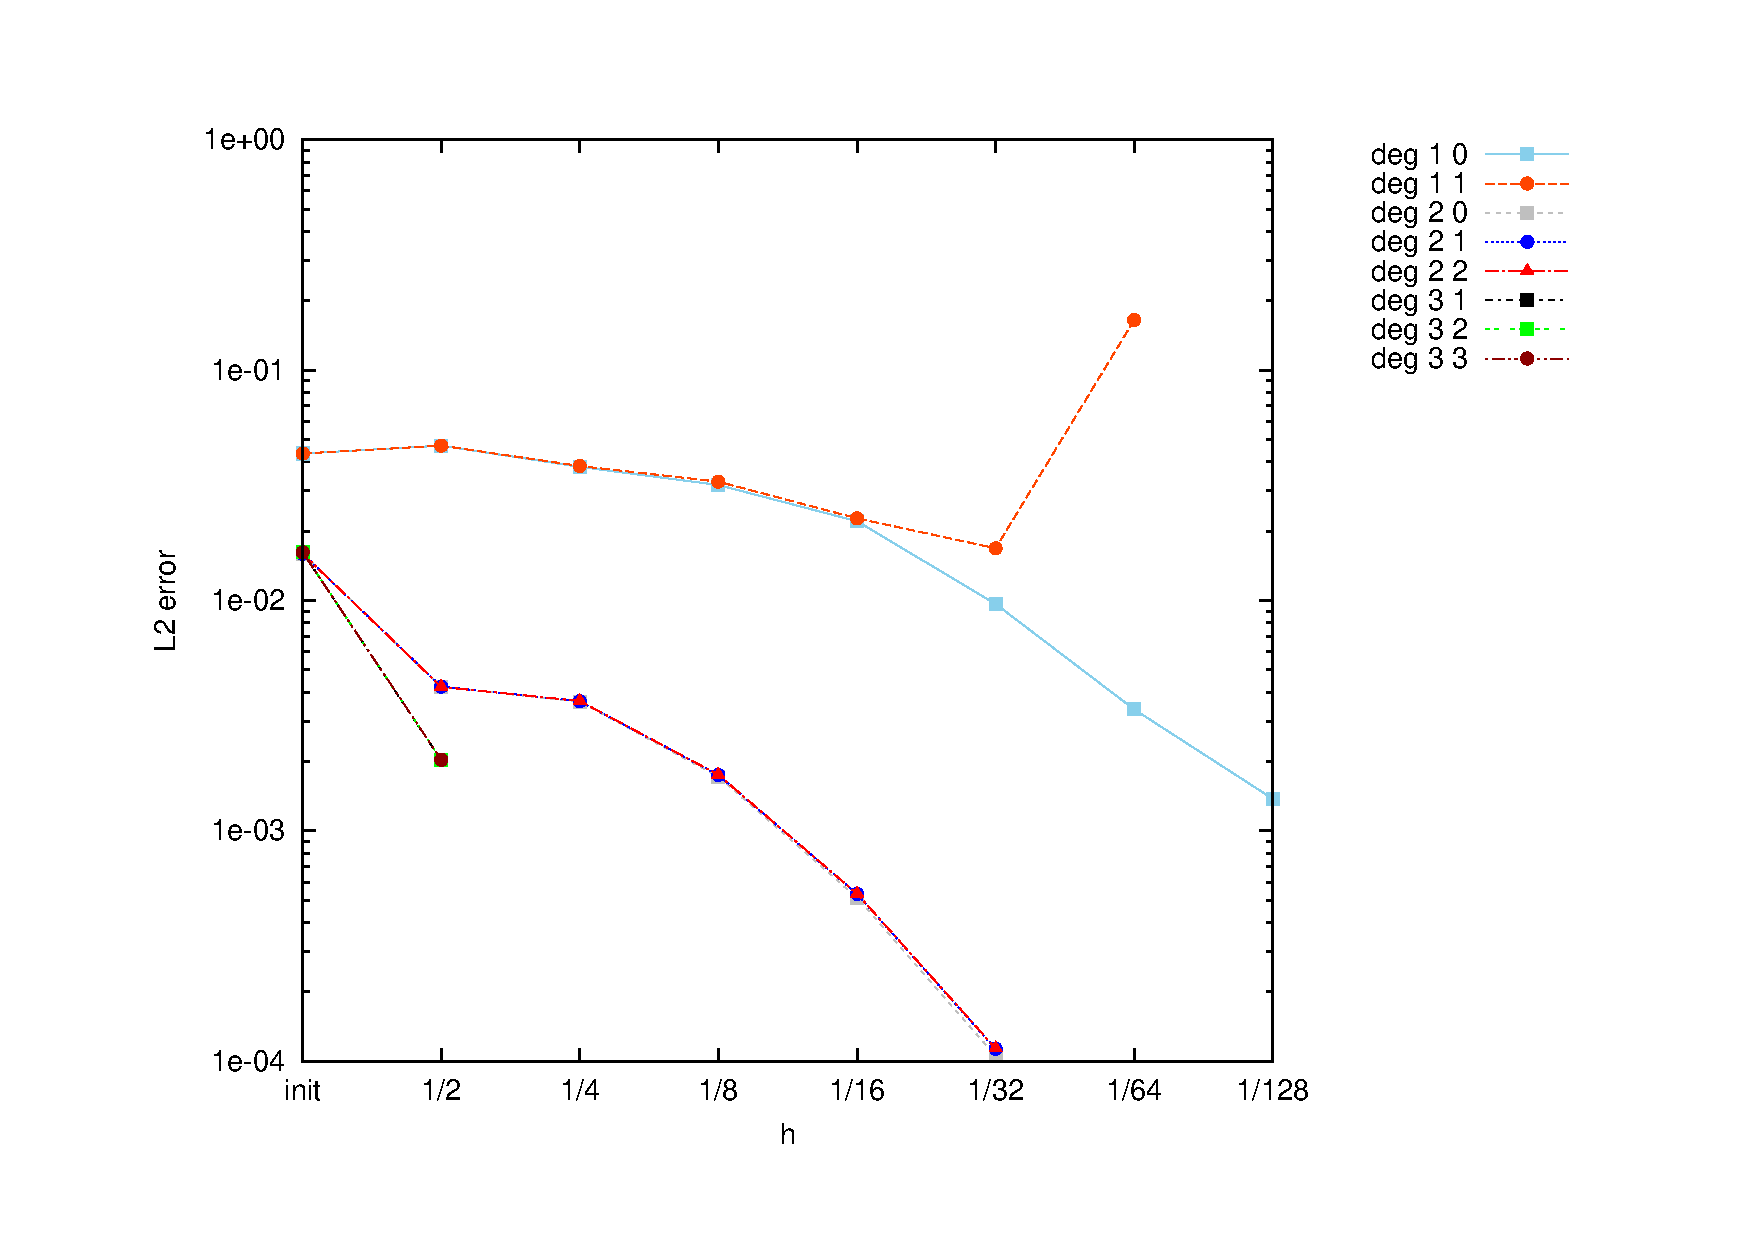
\includegraphics[scale =0.45]{plots/MA3_Neilan_GradJump_l2.pdf}
	\caption{$L^2$ errors for Test \ref{test singularity} and additional gradient jump penalty}
	\label{fig: l2 errors test 3 jump}
\end{figure}

\begin{figure}[H]
	\centering
	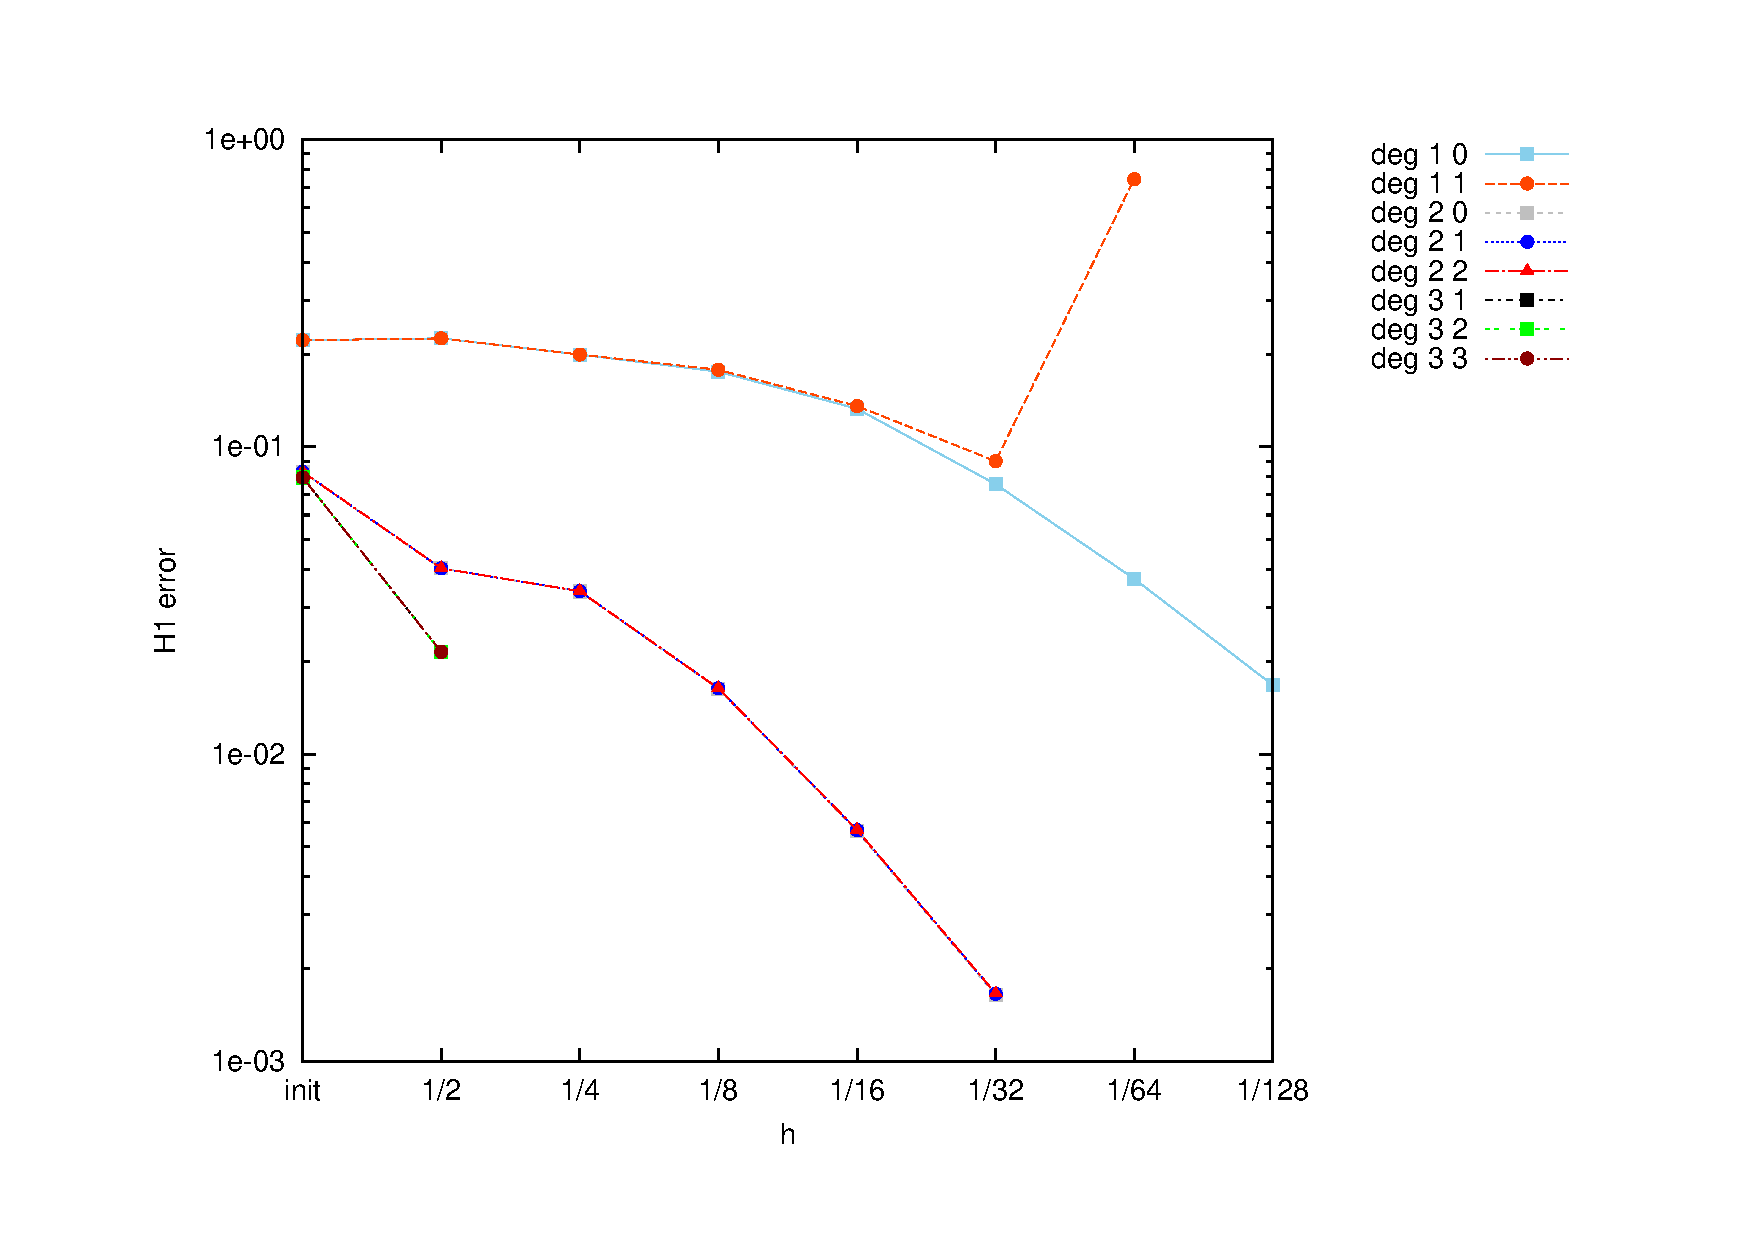
\includegraphics[scale =0.4]{plots/MA3_Neilan_GradJump_h1.pdf}
	\caption{$H^1$ errors for Test \ref{test singularity} and additional gradient jump penalty}
	\label{fig: h1 errors test 3 jump}
\end{figure}

\begin{table}[h]
\centering
	\begin{subtable}[b]{0.45\textwidth}
		\centering
		\pgfplotstabletypeset[columns={iterations, l2error, h1error,N},
		every row 0 column 0/.style={set content=init},
		]{\MAThreeJumpdegOneZero}
		\caption{Error for $k=1, k_{DH}=0$}
	\end{subtable}
	~
	\begin{subtable}[b]{0.45\textwidth}
		\centering
		\pgfplotstabletypeset[
		columns={iterations, l2error, h1error,N},
		every row 0 column 0/.style={set content=init},
		every row 6 column 1/.style={set content=-},
		every row 6 column 2/.style={set content=-},
		every row 6 column 3/.style={set content=-},
		every row 7 column 1/.style={set content=-},
		every row 7 column 2/.style={set content=-},
		every row 7 column 3/.style={set content=-},
		]{\MAThreeJumpdegTwoTwo}
		\caption{Error for $k=2, k_{DH}=2$}
	\end{subtable}
	\caption{Errors for Test \ref{test singularity} and additional gradient jump penalty}
	\label{tab: l2 errors test 3 jump}
\end{table}	

As in Test \ref{test smooth} the pair $k=1$ and $k_{DH}=1$ induces a unstable method. We further observe that the method with $k=2$ performs well on coarse grids, whereas for $k=3$ Newton's method does not converge on the coarsest grid. The numerical orders given in Table \ref{tab: order jump 3} show that the error decreases faster for quadratic polynomials during the first refinements. Yet, for grids with $h \geq \frac 1 {32}$ only the pairing $k=1$ and $k_{DH} =0$ yields convergence.

\begin{table}[h]
\centering
\begin{subtable}[b]{0.45\textwidth}
	\pgfplotstabletypeset
	{
		k $k_{DH}$ {numerical order}
		1 0 0.8565
		2 1 1.32222
		2 2 1.32048
	}
	\caption{Numerical order in $L^2$ norm}
	\end{subtable}
	\begin{subtable}[b]{0.45\textwidth}
	\pgfplotstabletypeset
	{
		k $k_{DH}$ {numerical order}
		1 0 0.618481
		2 1 1.17823
		2 2 1.17823
	}
	\caption{Numerical order in $H^1$ norm}
	\end{subtable}
	\caption{Numerical order with jump penalty in Test \ref{test singularity}}
\label{tab: order jump 3}
\end{table}

